\DiaryEntry{Dijkstra's Algorithm}{2020-04-20}{Algorithms}

Dijkstra's algorithm solves the single-source shortest path problem on a weighted, directed graph $G=(V,E)$ in the case that all edge weights are non-negative.

The algorithm keeps two data structures: A set $S$ of vertices and a min-priority queue $Q$. The algorithm is shown below.

\begin{Verbatim}[numbers=left, xleftmargin=5mm]
Dijkstra(G, w, s)
   Init-Single-Source(G,s)
   S = 0
   Q = G.V
   while Q is not empty
       u = Extract-min(Q)
       S = S + u
       for each vertex v adjacent to u
          relax(u,v,w)
\end{Verbatim}

Initially, \verb|Init-Single-Source| assigns a distance estimate $d$ of infinity and no parent to each vertex with the exception of the source vertex (Line 2) - this is the same as in the Bellman-Ford algorithm. Lines $3$ and $4$ initialize the set $S$ to empty and the min-priority queue $Q$ with all vertices.

Then we iterate over all elements of the min-priority queue (Line $5$): We take the vertex $u$ with the smallest distance estimate $u.d$ from the queue (line $6$) anf add it to $S$ (line $7$). Now we iterate over all vertices $v$ adjacent to $u$ (line $8$) and relax each edge $u-v$ (line $9$).

Note that the algorithm only adds vertices to $S$ (and never takes any from the set) and it only takes vertices from the min-priority queue $Q$ and never adds vertices to the qeue. However, the relaxation modifies the distance estimate and therefore the order of elements in the priority queue.

The algorithm is greedy in the sense that in every iteration it chooses the most promising vertex; i.e. the one with the smallest distance estimate. As the edge weights are positive, this greedy strategy seems to work.  

\paragraph{Example.} We continue with our example graph.

\begin{figure}[H]
\centering
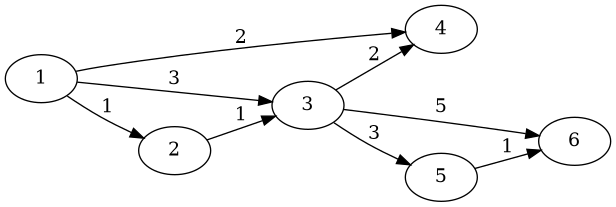
\includegraphics[scale=0.5]{images/dijkstra_1.png}
\end{figure}

Choosing vertex $1$ as source, \verb|Init-Single-Source| yields the following attribute vaues for each vertex.

\begin{figure}[H]
\centering
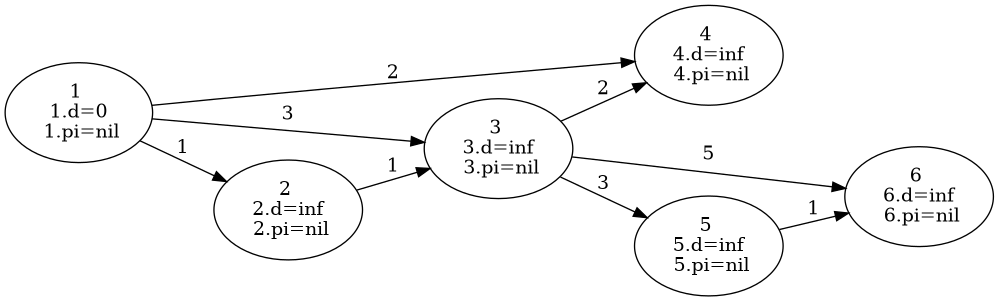
\includegraphics[scale=0.4]{images/dijkstra_2.png}
\end{figure}

Calling \verb|Extract-min| yields vertex $1$ (as it has the smallest distance estimate). Relaxing all edges (to vertices $2,3,$ and $4$, yields the following.

\begin{figure}[H]
\centering
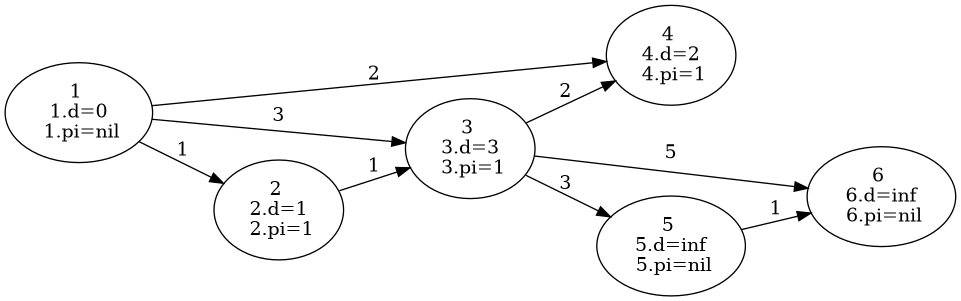
\includegraphics[scale=0.4]{images/dijkstra_3.png}
\end{figure}

The iteration is done and we retrieve the next element from the min-priority queue. The queue does no longer contain vertex $1$ (this was retrieved in the previous iteration), the vertex with smallest distance estimate is now vertex $2$. There is only one outgoing edge; relaxing it yields the following.

\begin{figure}[H]
\centering
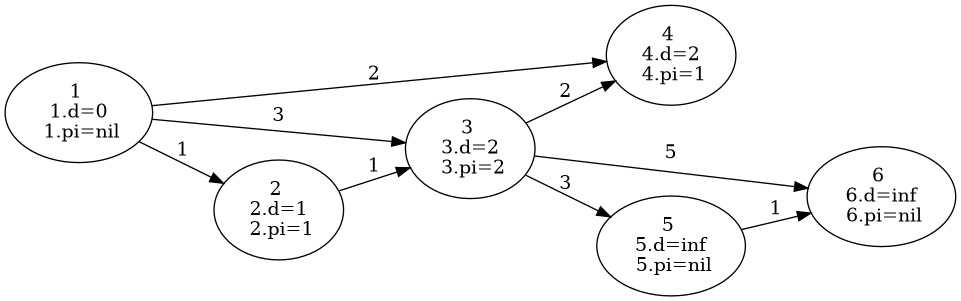
\includegraphics[scale=0.4]{images/dijkstra_4.png}
\end{figure}

Now the queue contains two vertices with minimum distance estimate $d=2$, namely vertex $3$ and vertex $4$. Since no edges leave vertex $4$, the algorithm does not do anything with this vertex and we continue with vertex $3$. Relaxing all edges leaving this vertex yields the following.

\begin{figure}[H]
\centering
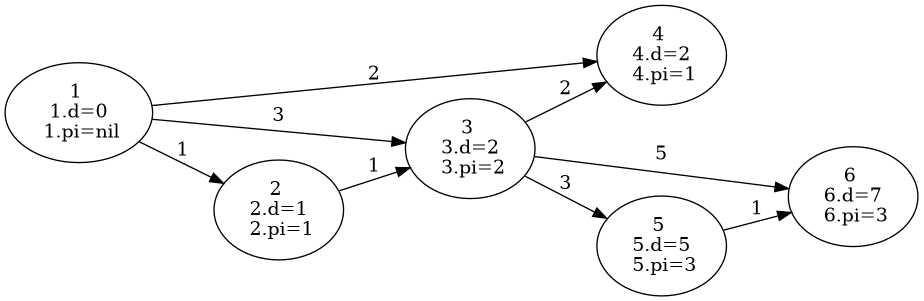
\includegraphics[scale=0.4]{images/dijkstra_5.png}
\end{figure}

We continue with vertex $5$ and relax the edge going to vertex $6$. This yields the following.

\begin{figure}[H]
\centering
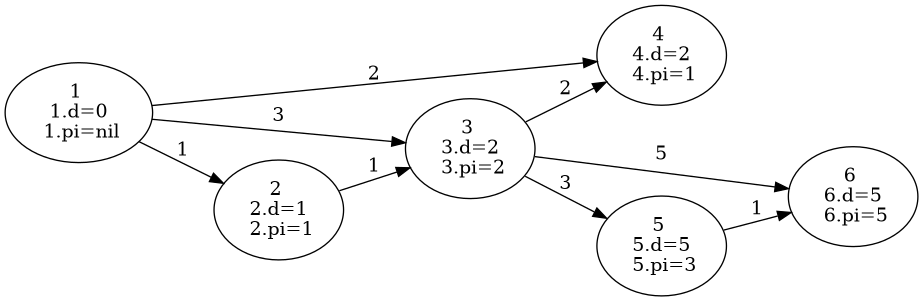
\includegraphics[scale=0.4]{images/dijkstra_6.png}
\end{figure}

The queue contains only vertex $6$, but since no edges leave it, the algorithm does not do anything. So, the algorithm stops with the above. If we color the edges of the tree with red, we arrive at the following presentation.

\begin{figure}[H]
\centering
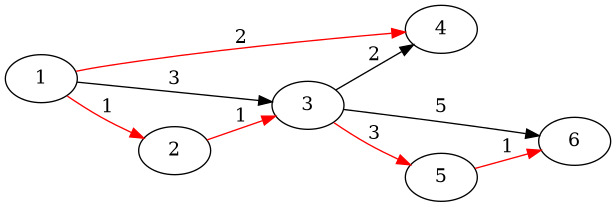
\includegraphics[scale=0.5]{images/sssp_2.png}
\end{figure}




%%% Local Variables:
%%% mode: latex
%%% TeX-master: "journal"
%%% End:
